\section{Casi d'uso}
\subsection{Scopo}
Lo scopo di questa sezione è la descrizione in elenco di tutti i casi d'uso individuati dal gruppo, in riferimento alle funzionalità dell'applicazione.
\subsection{Attori}
Come accordato con il proponente, non essendo richiesto alcun servizio di autenticazione e tantomeno la figura di un amministratore per la gestione del database, è presente un solo attore nella gerarchia: l'utente generico.

\begin{figure}[h]
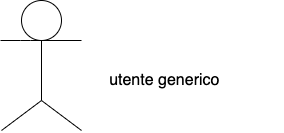
\includegraphics[width=1cm]{section/Images/Utente.png}
\centering
\caption{Gerarchia attori}
\end{figure}

\begin{description}
\item[Utente]:
Si riferisce all'utente generico che può accedere alla piattaforma e utilizzare tutti i servizi disponibili.
\end{description}

\newpage
\subsection{Elenco casi d'uso}
\subsubsection{UC1 - Caricamento del dataset}
\begin{figure}[h]
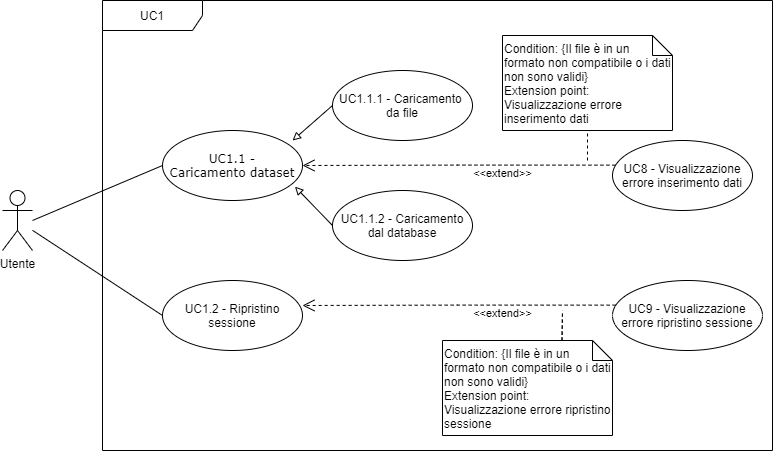
\includegraphics[width=\linewidth]{section/Images/UC1.png}
\centering
\caption{UC1 - Caricamento del dataset}
\end{figure}
\begin{itemize}
	\item \textbf{Attore primario}: Utente.
	\item \textbf{Precondizioni}: Il sistema è raggiungibile e funzionante.
	\item \textbf{Postcondizioni}: Viene visualizzato un messaggio che avvisa l'utente del corretto caricamento dei dati e della loro validità.
	\item \textbf{Scenario principale}:
		\begin{enumerate}
			\item L'utente accede al sistema;
			\item L'utente sceglie come ricavare i dati:
				\begin{enumerate}[(a)]
			\item L'utente seleziona la funzionalità "carica file" [UC1.1];
			\item L'utente seleziona un dataset tra quelli disponibili nel database [UC1.2].
				\end{enumerate}
		\end{enumerate}
	\item \textbf{Estensioni}:
	\begin{enumerate}[(a)]
		\item Nel caso in cui il file sia in un formato sbagliato o i dati non sono validi:
		\begin{enumerate}[1.]
			\item i dati non vengono caricati nel sistema;
			\item viene visualizzato un errore esplicativo [UC7].
		\end{enumerate}
	\end{enumerate}
\end{itemize}

\subsubsection{UC1.1 - Caricamento dataset da file}

\begin{itemize}
	\item \textbf{Attore primario}: Utente.
	\item \textbf{Precondizioni}: Il sistema è raggiungibile e funzionante. L'utente ha a disposizione un dataset in formato CSV.
	\item \textbf{Postcondizioni}: I dati presenti nel file vengono caricati nel sistema. Viene visualizzato un messaggio che avvisa l'utente del corretto caricamento e della validità dei dati.
	\item \textbf{Scenario principale}: L'utente sceglie di caricare un dataset personale o ricavato da altre fonti esterne.
	
\end{itemize}

\subsubsection{UC1.2 - Caricamento dataset dal database}

\begin{itemize}
	\item \textbf{Attore primario}: Utente.
	\item \textbf{Precondizioni}: Il sistema è raggiungibile e funzionante. L'utente effettua una query dal database disponibile per prelevare il dataset.
	\item \textbf{Postcondizioni}: I dati vengono caricati nel sistema. Viene visualizzato un messaggio che avvisa l'utente del corretto caricamento e della loro validità.
	\item \textbf{Scenario principale}: L'utente sceglie di caricare un dataset tra quelli presenti nel database.
	
\end{itemize}


  
\subsection{UC2 - Selezione delle dimensioni da utilizzare}
\begin{itemize}
	\item \textbf{Attore primario}: Utente;
	\item \textbf{Precondizioni}: L'utente ha caricato i dati nel sistema [UC1];
	\item \textbf{Postcondizioni}: Le dimensioni scelte vengono aggiornate nel sistema e i dati sono pronti per essere visualizzati [UC6];
	\item \textbf{Scenario principale}:
		\begin{enumerate}
			\item All'utente viene presentata una schermata con tutte le dimensioni presenti nel dataset caricato già selezionate di default;
			\item Per ogni dimensione è presente una cella da selezionare nel caso la si voglia utilizzare o meno;
			\item L'utente seleziona le dimensioni che desidera analizzare.
		\end{enumerate}
	\item \textbf{Estensioni:}
		\begin{enumerate}[(a)]
			\item Nel caso in cui l'utente non abbia selezionato nessuna dimensione:
			\begin{enumerate}[1.]
				\item Le dimensioni non vengono aggiornate nel sistema;
				\item Viene visualizzato un messaggio d'errore esplicativo [UC12].
			\end{enumerate}
		\end{enumerate}
\end{itemize}
\newpage
\subsection{UC6 - Personalizzazione della visualizzazione}
\begin{figure}[h]
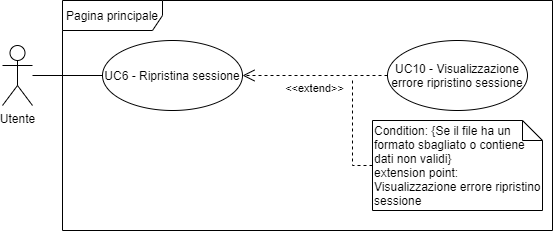
\includegraphics[width=\linewidth]{Section/Images/UC6.png}
\centering
\caption{Diagramma sulla personalizzazione della visualizzazione scelta}
\end{figure}
\begin{itemize}
	\item \textbf{Attore primario}: Utente;
	
	\item \textbf{Precondizioni}: L'utente ha scelto il grafico tra quelli a disposizione nel sistema [UC5];
	
	\item \textbf{Postcondizioni}: Il grafico viene aggiornato con le personalizzazioni impostate dall'utente;
	
	\item \textbf{Scenario principale}: L’utente sceglie come impostare le opzioni di personalizzazione del grafico. Verranno applicati, per ciascun campo, dei valori di default che l'utente può decidere di modificare o meno. In caso fosse stato precedentemente caricato un file di ripristino sessione [UC1.2] i valori di default iniziali diventerebbero quindi quelli specificati in questo file, lasciando comunque all'utente la possibilità di modificarli;
	
	\item \textbf{Generalizzazioni}: L'utente imposta i parametri di personalizzazione della visualizzazione scelta:
	\begin{enumerate}[(a)]
	\item Personalizzazione \textit{Scatter Plot Matrix} [UC6.1];
	\item Personalizzazione \textit{Adjacency Matrix} [UC6.2];
	\item Personalizzazione \textit{Force Field} [UC6.3];
	\item Personalizzazione \textit{Proiezione Lineare Multi Asse} [UC6.4];
	\item Personalizzazione \textit{Heat Map} [UC6.5].
	\end{enumerate}
		
\end{itemize}



